\chapter{MODELO PROPOSTO PARA ALOCAÇÃO DE PORTFÓLIOS}
\label{chapter:arquitetura}

Este capítulo apresenta o modelo proposto para integrar dados
de mercado e notícias financeiras à construção de carteiras.
A proposta utiliza previsões de aprendizado de máquina e sinais
de sentimento para formular visões sobre os ativos, incorporadas
ao modelo Black--Litterman de acordo com suas respectivas
incertezas.

Inicialmente, apresenta-se a organização geral do modelo.
Em seguida, são detalhadas a geração dos sinais quantitativos
e textuais, sua combinação na formulação das visões e a obtenção
dos pesos da carteira sob as restrições de investimento adotadas.

\section{Arquitetura Geral do Sistema}
\label{sec:arquitetura_geral}

A arquitetura proposta é organizada como um \textit{pipeline} híbrido que converte séries temporais de mercado e informações textuais em um vetor de pesos de carteira. O sistema combina sinais quantitativos, obtidos a partir de preços, volumes e indicadores derivados, com sinais qualitativos, extraídos de manchetes financeiras.

A utilização do modelo de Black--Litterman é motivada pela instabilidade frequentemente observada em carteiras construídas diretamente a partir de médias históricas de retorno. Como essas médias são estimadores sujeitos a elevada incerteza amostral, sua utilização direta na otimização média-variância pode resultar em alocações extremas e sensíveis a pequenas alterações nos dados. O modelo de Black--Litterman oferece uma alternativa ao combinar retornos de equilíbrio implícitos no mercado com opiniões adicionais, ponderadas de acordo com o nível de incerteza associado a cada uma delas.

Neste trabalho, as opiniões são geradas de forma algorítmica a partir de duas fontes de dados. A primeira corresponde ao fluxo de mercado, composto por cotações diárias de um universo fixo de ações líquidas negociadas na B3, pela série do índice Ibovespa e por variáveis macroeconômicas. Esse fluxo alimenta o componente quantitativo, que estima retornos
futuros para cada ativo em diferentes horizontes. Essas previsões
capturam sinais em distintas escalas temporais e, após conversão
para uma base temporal comum, fundamentam as visões utilizadas
pelo modelo Black--Litterman na alocação da carteira. A segunda fonte corresponde ao fluxo textual, composto por manchetes financeiras que são filtradas por relevância e classificadas semanticamente. A partir desses dados, o componente qualitativo produz, para cada ativo e data, um sinal contínuo de sentimento.

Por fim, os componentes são integrados em uma etapa de fusão
para construir o vetor de opiniões $\boldsymbol{Q}$ e a matriz
de incertezas $\boldsymbol{\Omega}$. Neste trabalho, adota-se
uma matriz diagonal, na qual cada opinião recebe uma medida
individual de incerteza. Essa escolha simplifica a estimação,
mas não considera possíveis relações entre os erros das
diferentes opiniões.

A previsão quantitativa constitui a base da opinião, enquanto o sentimento atua como um modulador informacional, cuja influência é habilitada quando há pelo menos uma manchete disponível para o ativo na data considerada.

Em seguida, o bloco Black--Litterman combina o \textit{prior}
de equilíbrio de mercado $\boldsymbol{\pi}$, obtido a partir
dos pesos de mercado e da matriz de covariância dos retornos,
com as opiniões algorítmicas. O resultado é o vetor posterior
de retornos esperados $\boldsymbol{\mu}$. Por fim, esse vetor
é utilizado na obtenção dos pesos preliminares da carteira,
posteriormente ajustados para impedir posições vendidas
(pesos negativos) e limitar a proporção do capital alocada
em cada ativo.
\begin{figure}[htbp]
    \centering
    \caption{Integração dos componentes do modelo proposto.}
    \label{fig:arquitetura_geral}

    \resizebox{0.6\textwidth}{!}{%
    \begin{tikzpicture}[
        node distance=0.45cm and 1.3cm,
        bloco/.style={
            draw,
            rounded corners=2pt,
            align=center,
            text width=4cm,
            minimum height=0.85cm,
            inner sep=6pt,
            font=\small
        },
        quantitativo/.style={
            bloco, fill=blue!5, draw=blue!60!black
        },
        textual/.style={
            bloco, fill=green!5, draw=green!50!black
        },
        integracao/.style={
            bloco, fill=purple!5, draw=purple!60!black
        },
        seta/.style={->, >=stealth, thick}
    ]

    \node[quantitativo] (dados)
        {Dados de mercado};

    \node[textual, right=of dados] (noticias)
        {Notícias financeiras};

    \node[quantitativo, below=of dados] (atributos)
        {Engenharia de atributos};

    \node[textual, below=of noticias] (llm)
        {Classificação por LLM\\
        em regime \textit{zero-shot}};

    % Mesma altura para os dois blocos de sinais
    \node[
        quantitativo,
        below=of atributos,
        minimum height=1.2cm
    ] (previsao)
        {Previsões de retorno\\
        XGBoost};

    \node[
        textual,
        below=of llm,
        minimum height=1.2cm
    ] (sentimento)
        {Agregação do sentimento\\
        $\psi$};

    % Centro abaixo do bloco mais baixo
    \path (previsao.south |- sentimento.south)
        -- (sentimento.south)
        coordinate[midway] (centro);

    \node[integracao, below=0.8cm of centro] (visoes)
        {Fusão dos sinais\\
        Opiniões $\boldsymbol{Q}$ e
        incertezas $\boldsymbol{\Omega}$};

    \node[integracao, below=of visoes] (bl)
        {Modelo Black--Litterman\\
        Retornos atualizados $\boldsymbol{\mu}$};

    \node[
        bloco,
        left=0.8cm of bl,
        text width=3.2cm,
        fill=gray!10
    ] (equilibrio)
        {Equilíbrio de mercado\\
        $\boldsymbol{\pi}$ e $\boldsymbol{\Sigma}$};

    \node[bloco, below=of bl] (pesos)
        {Pesos preliminares};

    \node[
        bloco,
        below=of pesos,
        fill=orange!10
    ] (ajustes)
        {Ajuste dos pesos\\
        Sem posições vendidas e\\
        com limite de concentração};

    \node[
        bloco,
        below=of ajustes,
        fill=gray!10
    ] (carteira)
        {Carteira final\\
        $\boldsymbol{w}^{\star}$};

    % Fluxos quantitativo e textual
    \draw[seta] (dados) -- (atributos);
    \draw[seta] (atributos) -- (previsao);
    \draw[seta] (noticias) -- (llm);
    \draw[seta] (llm) -- (sentimento);

    % Entradas distintas na borda superior da fusão
    \draw[seta]
        (previsao.south) -- ++(0,-0.25cm)
        -| ([xshift=-0.9cm]visoes.north);

    \draw[seta]
        (sentimento.south) -- ++(0,-0.25cm)
        -| ([xshift=0.9cm]visoes.north);

    % Rota externa: não atravessa o bloco de equilíbrio
    \coordinate (rotaexterna)
        at ([xshift=-0.5cm]equilibrio.west);

    \draw[seta]
        (dados.west)
        -- (dados.west -| rotaexterna)
        |- (equilibrio.west);

    % Combinação e alocação
    \draw[seta] (visoes.south) -- (bl.north);
    \draw[seta] (equilibrio.east) -- (bl.west);
    \draw[seta] (bl.south) -- (pesos.north);
    \draw[seta] (pesos.south) -- (ajustes.north);
    \draw[seta] (ajustes.south) -- (carteira.north);

    \end{tikzpicture}%
    }

    \par\smallskip
    Fonte: Elaborado pelo autor.
\end{figure}

A organização em camadas permite avaliar separadamente os
componentes quantitativo e textual, identificar sua contribuição
para a opinião final e controlar a confiança atribuída aos sinais.
Esse controle permite reduzir a influência de informações
associadas a maior incerteza, como ocorre quando há poucas
notícias disponíveis para um ativo.

O componente quantitativo estima retornos para horizontes de
5, 10 e 21 pregões, correspondentes a aproximadamente uma semana,
duas semanas e um mês. As opiniões resultantes são convertidas
para uma escala diária para compatibilizar as entradas do modelo
Black--Litterman. Essa conversão não implica negociações diárias enquanto o rebalanceamento da carteira é mensal, conforme detalhado no capítulo de procedimentos.

\section{Inteligência Quantitativa}
\label{sec:inteligencia_quantitativa}

A componente quantitativa tem como objetivo produzir, para cada ativo $i$ e para cada data $t$ elegível, uma estimativa do retorno prospectivo em um horizonte $h$. Para isso, são utilizados modelos de aprendizado de máquina capazes de representar relações não lineares entre atributos técnicos, medidas de risco e variáveis relativas ao mercado.

Como família de modelos preditivos, adota-se o \textit{gradient boosting} de árvores de decisão, implementado por meio do algoritmo XGBoost. Essa classe de modelos é adequada à utilização de atributos heterogêneos e permite representar interações não lineares entre variáveis. Além disso, apresenta flexibilidade para lidar com dados financeiros ruidosos e relações que não são necessariamente lineares. Em um experimento complementar, descrito no \hyperref[cap:procedimento_experimental]{Capítulo~\ref*{cap:procedimento_experimental}}, uma configuração do XGBoost é comparada a outros modelos de previsão de retorno.

\begin{figure}[htbp]
    \centering
    \caption{Arquitetura interna do modelo \textit{Gradient Boosting} (XGBoost) para estimativa de retorno.}
    \label{fig:arquitetura_xgboost}
    
    \vspace{0.5cm}
    \resizebox{0.95\textwidth}{!}{%
    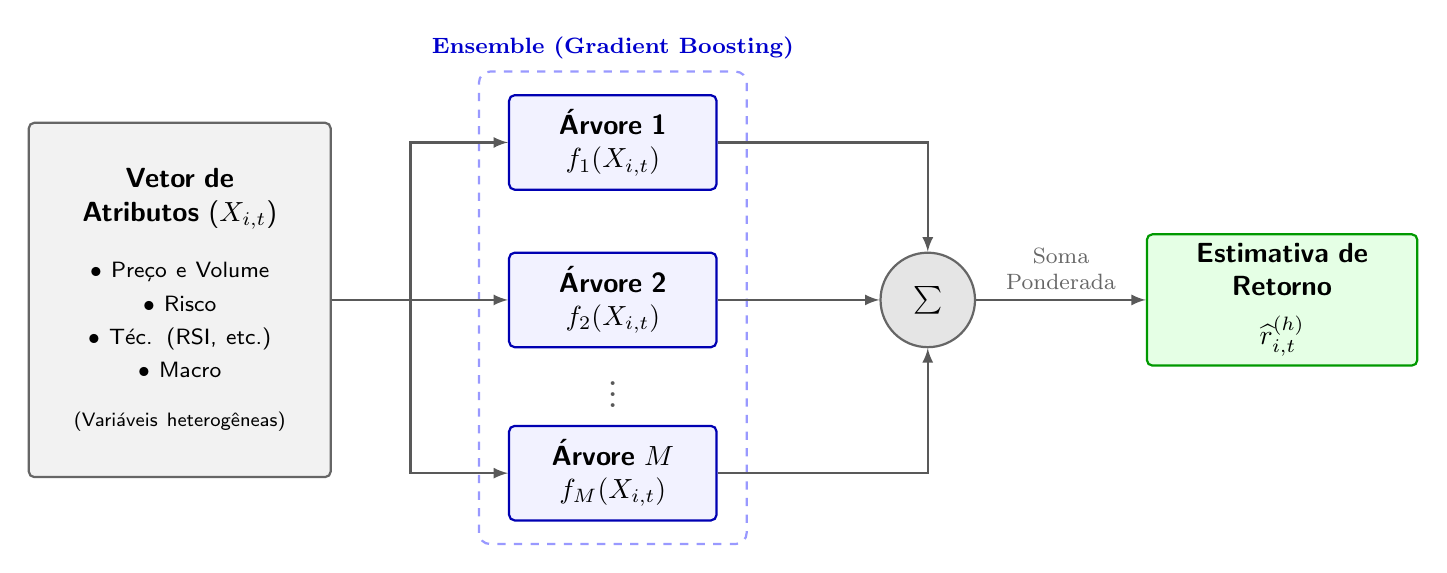
\begin{tikzpicture}[
        >=latex,
        font=\sffamily,
        % Estilos
        entrada/.style={draw=gray!80!black, thick, fill=gray!10, rounded corners=2pt, align=center, minimum height=4.5cm, text width=3.6cm},
        arvore/.style={draw=blue!70!black, thick, fill=blue!5, rounded corners=2pt, align=center, minimum height=1.2cm, text width=2.4cm},
        soma/.style={draw=gray!80!black, thick, circle, fill=gray!20, minimum size=1.2cm, inner sep=0pt, font=\Large\bfseries},
        saida/.style={draw=green!60!black, thick, fill=green!10, rounded corners=2pt, align=center, minimum height=1.5cm, text width=3.2cm},
        seta/.style={->, thick, gray!70!black}
    ]

        % 1. Vetor de Entrada
        \node[entrada] (X) at (0, 0) {
            \textbf{Vetor de}\\
            \textbf{Atributos} ($X_{i,t}$)\\[0.3cm]
            {\footnotesize $\bullet$ Preço e Volume}\\
            {\footnotesize $\bullet$ Risco}\\
            {\footnotesize $\bullet$ Téc. (RSI, etc.)}\\
            {\footnotesize $\bullet$ Macro}\\[0.2cm]
            {\scriptsize (Variáveis heterogêneas)}
        };

        % Caixa agrupadora para o Ensemble desenhada com coordenadas manuais (evita bugs do fit)
        \draw[draw=blue!40, dashed, thick, rounded corners] (3.8, -3.1) rectangle (7.2, 2.9);
        \node[font=\footnotesize\bfseries, text=blue!80!black] at (5.5, 3.2) {Ensemble (Gradient Boosting)};

        % 2. Árvores de Decisão (Ensemble)
        \node[arvore] (T1) at (5.5, 2.0) {\textbf{Árvore 1}\\ $f_1(X_{i,t})$};
        \node[arvore] (T2) at (5.5, 0) {\textbf{Árvore 2}\\ $f_2(X_{i,t})$};
        
        \node[font=\Large, text=gray!70!black] (pontos) at (5.5, -1.1) {$\vdots$};
        
        \node[arvore] (TM) at (5.5, -2.2) {\textbf{Árvore $M$}\\ $f_M(X_{i,t})$};

        % 3. Nó de Soma (Adição do Boosting)
        \node[soma] (Sum) at (9.5, 0) {$\sum$};

        % 4. Saída Final
        \node[saida] (Out) at (14, 0) {
            \textbf{Estimativa de}\\
            \textbf{Retorno}\\[0.2cm]
            $\boldsymbol{\widehat{r}_{i,t}^{(h)}}$
        };

        % Conexões Entrada -> Árvores
        \draw[seta] (X.east) -- ++(1,0) |- (T1.west);
        \draw[seta] (X.east) -- ++(1,0) |- (T2.west);
        \draw[seta] (X.east) -- ++(1,0) |- (TM.west);

        % Conexões Árvores -> Soma
        \draw[seta] (T1.east) -| (Sum.north);
        \draw[seta] (T2.east) -- (Sum.west);
        \draw[seta] (TM.east) -| (Sum.south);

        % Conexão Soma -> Saída com texto em duas linhas
        \draw[seta] (Sum.east) -- (Out.west) node[midway, above, font=\footnotesize, text=gray!80!black, align=center] {Soma\\Ponderada};

    \end{tikzpicture}%
    }
    
    \par\smallskip
    Fonte: Elaborado pelo autor
\end{figure}

\subsection{Universo, Dados e Engenharia de Atributos}
\label{subsec:universo_dados}

O conjunto de dados quantitativos é formado por séries de preços, volumes negociados, informações relativas ao mercado e, quando disponíveis, variáveis macroeconômicas auxiliares.

A partir das séries originais, são calculados retornos logarítmicos diários. Para o ativo $i$, o retorno observado entre as datas $t-1$ e $t$ é definido por:

\begin{equation}
    R_{i,t}
    =
    \ln\left(
        \frac{P_{i,t}}{P_{i,t-1}}
    \right),
    \label{eq:retorno_logaritmico}
\end{equation}

em que $P_{i,t}$ representa o preço de fechamento ajustado do ativo $i$ na data $t$.

A engenharia de atributos prioriza variáveis relativas, com o objetivo de reduzir o risco de vazamento do nível absoluto de preços e favorecer a capacidade de generalização do modelo. Entre os atributos utilizados estão defasagens de retornos, indicadores de momento, métricas de volatilidade, medidas de liquidez, osciladores técnicos e variáveis relativas ao índice de mercado.

A utilização de variáveis relativas permite comparar ativos com diferentes escalas de preço e diferentes níveis de volatilidade. Também são utilizadas múltiplas janelas retrospectivas, de modo que o modelo possa observar simultaneamente comportamentos de curto, médio e longo prazo.

Para uma janela móvel de comprimento $n$, o coeficiente beta do ativo $i$ em relação ao mercado $m$ é calculado por:

\begin{equation}
    \beta_{i,t}^{(n)}
    =
    \frac{
        \widehat{\operatorname{Cov}}_{n}
        \left(
            R_i,R_m
        \right)
    }{
        \widehat{\operatorname{Var}}_{n}
        \left(
            R_m
        \right)
    },
    \label{eq:beta_rolling}
\end{equation}

em que $R_i$ e $R_m$ representam, respectivamente, os retornos do ativo $i$ e do mercado, enquanto $\widehat{\operatorname{Cov}}_{n}$ e $\widehat{\operatorname{Var}}_{n}$ representam os estimadores amostrais de covariância e variância calculados na janela de tamanho $n$.

Também podem ser calculadas medidas de excesso de retorno, escores padronizados e diferenças entre a volatilidade do ativo e a volatilidade do mercado. A utilização conjunta dessas variáveis permite ao modelo identificar tanto efeitos de continuidade de tendência quanto possíveis movimentos de reversão.

\subsection{Variável-Alvo e Horizontes Concorrentes}
\label{subsec:variavel_alvo}

A variável-alvo é definida como o retorno logarítmico prospectivo do ativo $i$ em um horizonte $h$:

\begin{equation}
    y_{i,t}^{(h)}
    =
    \ln\left(
        \frac{P_{i,t+h}}{P_{i,t}}
    \right),
    \label{eq:target_return}
\end{equation}

em que $P_{i,t}$ representa o preço de fechamento ajustado do ativo $i$ na data $t$, e $h$ representa o horizonte de previsão em dias úteis.

Neste trabalho, são avaliados os horizontes:

\begin{equation}
    h\in\{5,10,21\}.
    \label{eq:horizontes}
\end{equation}

Esses valores representam, respectivamente, aproximadamente uma semana, duas semanas e um mês de negociação. Para cada horizonte, é treinado um modelo conjunto com os dados dos 20 ativos. A escolha do horizonte vencedor é realizada individualmente para cada ativo com base no desempenho direcional obtido fora da amostra, utilizando previsões \textit{out-of-fold}.

A acurácia direcional é calculada pela proporção de observações nas quais o modelo identifica corretamente o sinal do retorno futuro:

\begin{equation}
    \widehat{a}_{i,t}^{(h)}
    =
    \frac{1}{M}
    \sum_{k=1}^{M}
    \mathbb{I}
    \left[
        \operatorname{sign}
        \left(
            \widehat{y}_{i,k}^{(h)}
        \right)
        =
        \operatorname{sign}
        \left(
            y_{i,k}^{(h)}
        \right)
    \right],
    \label{eq:acuracia_direcional}
\end{equation}

em que $M$ representa o número de observações avaliadas, $\widehat{y}_{i,k}^{(h)}$ representa a previsão do modelo e $\mathbb{I}[\cdot]$ representa a função indicadora.

A seleção do horizonte é realizada exclusivamente com base nas previsões da validação de 2024 cujos retornos já eram conhecidos antes de 2025. O conjunto de teste permanece separado até a avaliação final, evitando que a escolha do horizonte introduza viés otimista nos resultados.

Quando a acurácia direcional do modelo selecionado é inferior a $52\%$, sua confiança é reduzida por meio de um fator de penalização incorporado ao cálculo da matriz $\boldsymbol{\Omega}$. Esse procedimento não elimina necessariamente o sinal quantitativo, mas reduz sua influência na atualização posterior do modelo Black--Litterman.

\subsection{Aprendizado, Validação \textit{Walk-Forward} e Calibração}
\label{subsec:aprendizagem_validacao}

O treinamento dos modelos emprega validação temporal do tipo \textit{walk-forward}, também denominada validação cruzada temporal expansiva. Nesse procedimento, o modelo é treinado em uma janela histórica e avaliado em um período posterior. Após cada etapa, a janela de treinamento é expandida para incorporar novas observações.

A estrutura temporal é necessária porque a utilização de uma validação aleatória convencional poderia misturar observações passadas e futuras, produzindo uma estimativa excessivamente otimista do desempenho. Além disso, como os retornos prospectivos de diferentes datas podem se sobrepor, é utilizado um intervalo de separação entre os períodos de treinamento e teste.

Para evitar o vazamento de informação decorrente da sobreposição das janelas de retorno, impõe-se um \textit{embargo} de comprimento $h$ entre o final do conjunto de treinamento e o início do conjunto de teste. O procedimento é ilustrado na ~\ref{fig:walk_forward}.

\begin{figure}[htbp]
    \centering
    \caption{Esquema de particionamento \textit{walk-forward} com embargo temporal.}
    \label{fig:walk_forward}

    \resizebox{0.85\textwidth}{!}{%
    \begin{tikzpicture}

        \def\foldheight{0.6}
        \def\foldspacing{1.2}

        \foreach \i in {1,2,3} {

            \pgfmathsetmacro{\y}{-\i * \foldspacing}

            \draw[
                ->,
                thick,
                gray
            ]
            (0,{\y-0.4})
            --
            (12,{\y-0.4})
            node[
                right,
                font=\scriptsize
            ] {Tempo};

            \node[
                anchor=east,
                font=\bfseries
            ]
            at (-0.5,{\y+\foldheight/2})
            {\textit{Fold} \i};

            \pgfmathsetmacro{\trainwidth}{4+\i*1.5}

            \draw[
                fill=blue!20,
                draw=blue!80!black,
                thick
            ]
            (0,\y)
            rectangle
            (\trainwidth,{\y+\foldheight});

            \node[
                font=\small
            ]
            at ({\trainwidth/2},{\y+\foldheight/2})
            {Treino};

            \pgfmathsetmacro{\embargowidth}{1}

            \draw[
                fill=red!20,
                draw=red!80!black,
                thick,
                pattern=north east lines,
                pattern color=red!40
            ]
            (\trainwidth,\y)
            rectangle
            ({\trainwidth+\embargowidth},{\y+\foldheight});

            \node[
                font=\scriptsize,
                align=center
            ]
            at (
                {\trainwidth+\embargowidth/2},
                {\y+\foldheight/2}
            )
            {Gap\\($h$)};

            \pgfmathsetmacro{\testwidth}{2}

            \draw[
                fill=green!20,
                draw=green!80!black,
                thick
            ]
            ({\trainwidth+\embargowidth},\y)
            rectangle
            (
                {\trainwidth+\embargowidth+\testwidth},
                {\y+\foldheight}
            );

            \node[
                font=\small
            ]
            at (
                {\trainwidth+\embargowidth+\testwidth/2},
                {\y+\foldheight/2}
            )
            {Teste OOF};
        }

    \end{tikzpicture}
    }

    \par\smallskip
    Fonte: Elaborado pelo autor
\end{figure}

Durante o treinamento, as observações mais recentes recebem maior peso por meio de um decaimento exponencial. Essa ponderação parte da hipótese de que as condições recentes de mercado podem ser mais representativas do regime atual do que observações muito antigas.

O componente quantitativo estabelece uma competição interna entre um regressor, que produz diretamente uma estimativa contínua de retorno, e um classificador de três regimes, que classifica o retorno futuro como queda, neutralidade ou alta.

Quando o regressor é selecionado, sua saída é utilizada diretamente como estimativa de retorno. Quando o classificador é selecionado, as probabilidades previstas para cada regime são convertidas em uma expectativa de retorno por meio de:

\begin{equation}
    \widehat{r}_{i,t}^{(h)}
    =
    \boldsymbol{p}_{i,t}^{\top}
    \boldsymbol{\mu}_{i,t}^{\mathrm{regime}},
    \label{eq:expected_return_class}
\end{equation}

em que $\boldsymbol{p}_{i,t}$ representa o vetor de probabilidades preditas para os três regimes e $\boldsymbol{\mu}_{i,t}^{\mathrm{regime}}$ representa o vetor das médias condicionais de retorno observadas no conjunto de treinamento para cada regime.

O resultado desse processo é uma previsão quantitativa de retorno que será posteriormente convertida para a escala diária e utilizada na construção do vetor de opiniões $\boldsymbol{Q}$.

\section{Inteligência Qualitativa}
\label{sec:inteligencia_qualitativa}

A componente qualitativa parte da hipótese de que manchetes financeiras podem condensar expectativas, eventos corporativos e choques informacionais que ainda não foram completamente incorporados aos preços. O objetivo dessa etapa é transformar textos jornalísticos em um sinal escalar diário, limitado em magnitude e ponderado pela quantidade de evidências textuais disponíveis.

\subsection{Coleta, Filtragem e Unidade de Análise}
\label{subsec:coleta_filtragem}

As manchetes são coletadas a partir de agregadores de notícias e fontes estruturadas, como feeds RSS. Após a coleta, os textos são submetidos a etapas de higienização, que incluem a remoção de duplicatas, a padronização de caracteres e o descarte de títulos genéricos ou sem relação explícita com uma empresa ou ativo do universo analisado.

Para evitar viés de antecipação, somente manchetes publicadas até o horário de formação da carteira são utilizadas na construção do sinal da data $t$. Notícias publicadas posteriormente são consideradas apenas em datas subsequentes.

A unidade metodológica de agregação é a empresa econômica. Dessa forma, ativos distintos pertencentes à mesma companhia, como ações ordinárias e preferenciais, compartilham o mesmo conjunto de notícias. Essa decisão evita a fragmentação artificial da evidência textual e permite que um evento corporativo seja associado de maneira consistente aos diferentes ativos emitidos pela mesma empresa.

Seja $\mathcal{N}_{i,t}$ o conjunto de manchetes associadas ao ativo ou à empresa do ativo $i$ na data $t$. O número de manchetes disponíveis é definido por:

\begin{equation}
    n_{i,t}
    =
    \left|
        \mathcal{N}_{i,t}
    \right|.
    \label{eq:numero_noticias}
\end{equation}

\begin{figure}[htbp]
    \centering
    \caption{Fluxo simplificado de processamento da inteligência qualitativa.}
    \label{fig:esteira_qualitativa}
    
    \vspace{0.3cm}
    \resizebox{\textwidth}{!}{%
    \begin{tikzpicture}[
        >=latex,
        font=\sffamily,
        bloco/.style={draw=black!70, thick, rounded corners=3pt, align=center, inner sep=10pt, minimum height=3.8cm},
        seta/.style={->, ultra thick, gray!80, line width=1.5pt}
    ]

        % 1. Coleta
        \node[bloco, fill=gray!10, text width=2.8cm] (coleta) at (0, 0) {
            \textbf{1. Coleta}\\[10pt]
            Agregadores de notícias e\\ \textit{feeds} RSS
        };

        % 2. Higienização
        \node[bloco, fill=gray!10, text width=4.2cm, right=0.6cm of coleta] (higienizacao) {
            \textbf{2. Higienização}\\[10pt]
            \parbox{3.8cm}{\footnotesize
            \textbullet~ Remoção de duplicatas\\[4pt]
            \textbullet~ Padronização de caracteres\\[4pt]
            \textbullet~ Descarte de genéricos\\[4pt]
            \textbullet~ Filtro temporal ($< t$)}
        };

        % 3. Agregação
        \node[bloco, fill=blue!10, draw=blue!70!black, text width=3.8cm, right=0.6cm of higienizacao] (agregacao) {
            \textbf{3. Agregação por}\\[2pt]
            \textbf{Empresa Econômica}\\[10pt]
            {\footnotesize Ativos da mesma companhia (ON, PN) compartilham o sinal.}
        };

        % 4. Saída
        \node[bloco, fill=green!10, draw=green!70!black, text width=3.2cm, right=0.6cm of agregacao] (saida) {
            \textbf{4. Mensuração}\\[10pt]
            Conjunto $\mathcal{N}_{i,t}$\\[10pt]
            $\boldsymbol{n_{i,t} = |\mathcal{N}_{i,t}|}$
        };

        % Setas de conexão
        \draw[seta] (coleta.east) -- (higienizacao.west);
        \draw[seta] (higienizacao.east) -- (agregacao.west);
        \draw[seta] (agregacao.east) -- (saida.west);

    \end{tikzpicture}%
    }
    \par\smallskip
    Fonte: Elaborado pelo autor
\end{figure}

\subsection{Rotulação por Modelos de Linguagem}
\label{subsec:rotulacao_llms}

Cada manchete elegível é submetida a um Modelo de Linguagem de Grande Escala, denominado LLM. Mediante uma instrução do tipo \textit{zero-shot}, o modelo classifica o impacto esperado da notícia sobre a empresa ou sobre o ativo em uma das seguintes categorias: positivo, negativo ou neutro.

Define-se a função de conversão dos rótulos em escores numéricos por:

\begin{equation}
    s(\ell)
    =
    \begin{cases}
        +1,
        & \text{se } \ell=\text{positivo},\\
        -1,
        & \text{se } \ell=\text{negativo},\\
        0,
        & \text{se } \ell=\text{neutro}.
    \end{cases}
    \label{eq:mapa_sentimento}
\end{equation}

A média dos escores das manchetes disponíveis para o ativo $i$ na data $t$ é definida por:

\begin{equation}
    \overline{s}_{i,t}
    =
    \begin{cases}
        \displaystyle
        \frac{1}{n_{i,t}}
        \sum_{\ell\in\mathcal{N}_{i,t}}
        s(\ell),
        & \text{se } n_{i,t}>0,\\[1.2em]
        0,
        & \text{se } n_{i,t}=0.
    \end{cases}
    \label{eq:media_sentimento}
\end{equation}

Quando não há manchetes elegíveis para determinado ativo e data, atribui-se $\overline{s}_{i,t}=0$ exclusivamente para fins operacionais. Essa atribuição não representa evidência de neutralidade, mas ausência de informação textual disponível. A distinção é importante porque a ausência de notícias deve reduzir a influência do componente qualitativo, e não ser interpretada como uma manifestação observada de sentimento neutro.

\subsection{Compressão em Sinal Contínuo}
\label{subsec:compressao_sinal}

A média de sentimento isolada não diferencia adequadamente dias de cobertura escassa e dias de elevada repercussão midiática. Para incorporar a quantidade de evidências textuais e, simultaneamente, impedir que um grande volume de manchetes produza valores excessivamente elevados, utiliza-se a seguinte função de compressão:

\begin{equation}
    \psi_{i,t}
    =
    \tanh
    \left(
        \overline{s}_{i,t}
        \ln(1+n_{i,t})
    \right),
    \label{eq:sinal_continuo}
\end{equation}

em que $\psi_{i,t}\in(-1,1)$ representa o sinal contínuo de sentimento agregado.

A função tangente hiperbólica garante que o sinal permaneça limitado em magnitude. O termo $\ln(1+n_{i,t})$ incorpora a quantidade de manchetes com efeito marginal decrescente, evitando que eventos com elevada repercussão midiática dominem mecanicamente o processo de otimização.

\section{Otimização Híbrida via Black--Litterman}
\label{sec:otimizacao_hibrida}

O núcleo do sistema utiliza o modelo Black--Litterman para combinar os retornos de equilíbrio implícitos no mercado com as opiniões geradas pelos components quantitativo e qualitativo.

Considerando opiniões absolutas para todos os ativos, adota-se:

\begin{equation}
    \boldsymbol{P}
    =
    \boldsymbol{I}_{N},
    \label{eq:matriz_p}
\end{equation}

em que $\boldsymbol{I}_{N}$ representa a matriz identidade de dimensão $N$, correspondente ao número de ativos analisados.

O vetor posterior de retornos esperados é obtido por:

\begin{equation}
    \boldsymbol{\mu}_t
    =
    \left[
        \left(
            \tau\boldsymbol{\Sigma}_t
        \right)^{-1}
        +
        \boldsymbol{P}^{\top}
        \boldsymbol{\Omega}_t^{-1}
        \boldsymbol{P}
    \right]^{-1}
    \left[
        \left(
            \tau\boldsymbol{\Sigma}_t
        \right)^{-1}
        \boldsymbol{\pi}_t
        +
        \boldsymbol{P}^{\top}
        \boldsymbol{\Omega}_t^{-1}
        \boldsymbol{Q}_t
    \right],
    \label{eq:bl_mu_update}
\end{equation}

em que $\tau$ representa o fator de incerteza associado ao \textit{prior} de equilíbrio, $\boldsymbol{\Sigma}_t$ representa a matriz de covariância dos retornos, $\boldsymbol{\pi}_t$ representa o vetor de retornos de equilíbrio, $\boldsymbol{Q}_t$ representa o vetor de opiniões e $\boldsymbol{\Omega}_t$ representa a matriz de incertezas associadas às opiniões.

A ~\ref{fig:black_litterman_idzorek} ilustra a intuição do processo de atualização, detalhando a fusão entre a distribuição de equilíbrio e as opiniões submetidas.

\begin{figure}[H]
    \centering
    \caption{Derivação do novo vetor de retornos combinados no modelo Black-Litterman}
    \vspace{0.2cm}
    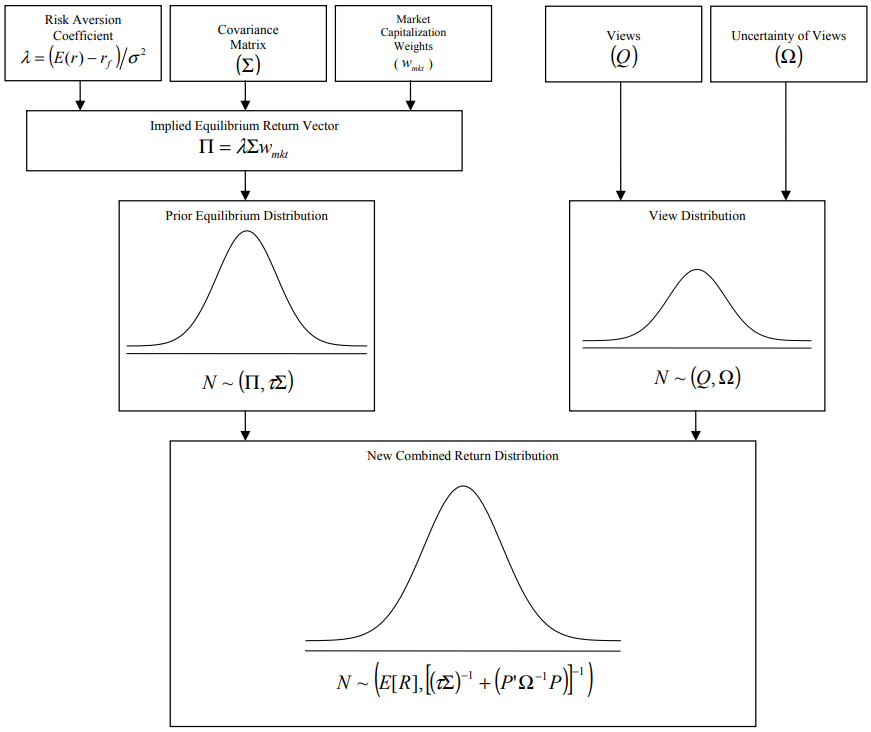
\includegraphics[width=0.9\textwidth]{03_Arquitetura/figures/BL idzorek 2005.png}
    \vspace{0.2cm}
    \\Fonte: {\cite{idzorek2005}.}
    \label{fig:black_litterman_idzorek}
\end{figure}

A inovação metodológica do sistema está na formulação dinâmica dos vetores e matrizes utilizados na atualização. O vetor $\boldsymbol{Q}_t$ combina previsões quantitativas e informações textuais, enquanto a matriz $\boldsymbol{\Omega}_t$ incorpora tanto a qualidade preditiva dos modelos quanto a quantidade de evidências disponíveis.

\subsection{Integração de Sinais no Vetor $\boldsymbol{Q}$ e Regra de \textit{Gate} de Notícias}
\label{subsec:integracao_gate}

Como o sentimento $\psi_{i,t}$ é adimensional, sua combinação com uma previsão de retorno requer um mapeamento para a escala de volatilidade típica do ativo.

Adota-se a média dos valores absolutos dos retornos nos
14 pregões anteriores como referência da magnitude recente
das variações do ativo. A janela é uma escolha de modelagem,
sem pressupor que seja ótima:

\begin{equation}
    \sigma_{i,t}^{\mathrm{ret}}
    =
    \frac{1}{14}
    \sum_{k=1}^{14}
    \left|
        \qquad R_{i,t-k}
    \right|.
    \label{eq:volatilidade_local}
\end{equation}

O sentimento é multiplicado por essa medida para tornar sua
magnitude compatível com a previsão de retorno, preservando
sua direção:

\begin{equation}
    \widetilde{\psi}_{i,t}
    =
    \psi_{i,t}
    \sigma_{i,t}^{\mathrm{ret}}.
    \label{eq:sentimento_reescalonado}
\end{equation}

O reescalonamento ajusta a magnitude do sentimento à escala
dos retornos recentes do ativo, preservando sua direção
positiva ou negativa.

Para evitar distorções causadas por escassez de notícias, define-se o coeficiente de cobertura, denominado \textit{gate} de notícias, por:

\begin{equation}
    c_{i,t}
    =
    \min
    \left(
        1,
        \frac{n_{i,t}}{n_{\min}}
    \right),
    \label{eq:gate_cobertura}
\end{equation}

\noindent em que $n_{\min}$ representa o número mínimo de manchetes considerado necessário para que o componente textual atinja sua influência máxima. Neste trabalho, adota-se $n_{\min}=3$ manchetes por ativo e dia. Assim, $c_{i,t}=0$ quando não há notícias e $c_{i,t}=1$ quando há pelo menos três manchetes disponíveis.

O comportamento do \textit{gate} é ilustrado na ~\ref{fig:gate_noticias}.

\begin{figure}[htbp]
    \centering
    \caption{Dinâmica do \textit{gate} de notícias ($c$) em relação à quantidade de manchetes ($n$).}
    \label{fig:gate_noticias}
    \vspace{0.2cm}

    \begin{tikzpicture}[
        >=Stealth, 
        scale=1.5,
        eixo/.style={->, thick, draw=gray!80!black},
        linha_guia/.style={dashed, draw=gray!50, thick},
        funcao/.style={ultra thick, draw=blue!70!black},
        texto_anotacao/.style={font=\footnotesize, text=gray!70!black, align=center}
    ]

        % 1. Preenchimento suave abaixo da curva (destaque visual)
        \fill[blue!5] (0,0) -- (1,1) -- (6.4,1) -- (6.4,0) -- cycle;

        % 2. Eixos
        \draw[eixo] (-0.2,0) -- (6.8,0) node[right, font=\small, text=black] {$n_{i,t}$ (Manchetes)};
        \draw[eixo] (0,-0.2) -- (0,1.5) node[above, font=\small, text=black] {$c_{i,t}$ (Cobertura)};

        % 3. Linhas de Guia (pontilhadas)
        \draw[linha_guia] (1,0) -- (1,1);
        \draw[linha_guia] (0,1) -- (1,1);

        % 4. Linha Principal da Função (Gate)
        \draw[funcao] (0,0) -- (1,1) -- (6.4,1);

        % 5. Marcador no ponto de saturação (inflexão)
        \filldraw[blue!70!black] (1,1) circle (1.5pt);
        \filldraw[blue!70!black] (0,0) circle (1.5pt);

        % 6. Ticks (Marcadores nos eixos)
        \draw[thick, gray!80!black] (1,0.05) -- (1,-0.05) node[below, text=black, font=\small] {$n_{\min}=3$};
        \draw[thick, gray!80!black] (0.05,1) -- (-0.05,1) node[left, text=black, font=\small] {$1{,}0$};

        % 7. Anotações de Texto
        % Indicação do ponto de cobertura integral
        \node[texto_anotacao, anchor=west] at (1.4, 0.5) {Cobertura integral\\a partir de 3 manchetes};
        
        % Texto de saturação repousando sobre a linha plana
        \node[texto_anotacao, anchor=south] at (5.7, 1.05) {Saturação\\($c=1$)};

    \end{tikzpicture}

    \par\smallskip
    Fonte: Elaborado pelo autor
\end{figure}

A previsão quantitativa é originalmente produzida para um horizonte $h$. Para que possa ser combinada com o sinal textual diário, ela é convertida para a escala diária por:

\begin{equation}
    q_{i,t}^{\mathrm{quant}}
    =
    \frac{
        \widehat{r}_{i,t}^{(h)}
    }{h}.
    \label{eq:quant_daily}
\end{equation}

A opinião híbrida diária é então definida por:

\begin{equation}
    Q_{i,t}
    =
    \left[
        \alpha
        +
        (1-\alpha)(1-c_{i,t})
    \right]
    q_{i,t}^{\mathrm{quant}}
    +
    (1-\alpha)c_{i,t}
    \widetilde{\psi}_{i,t},
    \label{eq:view_hibrida}
\end{equation}

\noindent em que $\alpha\in[0,1]$ representa o peso estrutural atribuído ao componente quantitativo quando a cobertura textual atinge o nível máximo.

A formulação possui três comportamentos importantes. Quando não há notícias, isto é, quando $c_{i,t}=0$, a opinião é composta exclusivamente pelo sinal quantitativo:

\begin{equation}
    Q_{i,t}
    =
    q_{i,t}^{\mathrm{quant}}.
    \label{eq:view_sem_noticias}
\end{equation}

Quando a cobertura atinge o limiar definido por $n_{\min}$, isto é, quando $c_{i,t}=1$, a opinião assume a combinação estrutural entre os componentes:

\begin{equation}
    Q_{i,t}
    =
    \alpha q_{i,t}^{\mathrm{quant}}
    +
    (1-\alpha)\widetilde{\psi}_{i,t}.
    \label{eq:view_cobertura_maxima}
\end{equation}

Adota-se $n_{\min}=3$ para reduzir a influência do sentimento
quando há poucas notícias. Adota-se esse valor de $n_{\min}$,  a partir de uma análise de sensibilidade com limites de uma a cinco manchetes nos resultados de 2025. Esse parâmetro reduz a influência do sentimento quando há poucas notícias: uma ou duas manchetes permitem participação parcial do componente textual, enquanto três ou mais habilitam a combinação integral.

\subsection{Cálculo Dinâmico da Matriz de Incerteza}
\label{subsec:calculo_omega}

A matriz $\boldsymbol{\Omega}$ representa a incerteza associada às opiniões utilizadas pelo modelo Black--Litterman. Quanto maior a incerteza associada a uma opinião, menor deve ser sua influência sobre o retorno posterior.

A confiança no modelo quantitativo é calculada com base no erro preditivo recente e em uma escala robusta de normalização. Define-se:

\begin{equation}
    c_{i,t}^{\mathrm{model}}
    =
    \kappa_{i,t}^{\mathrm{acc}}
    \exp
    \left(
        -\frac{e_{i,t}}{\xi_{i,t}}
    \right),
    \label{eq:confianca_modelo}
\end{equation}

\noindent em que $e_{i,t}$ representa o erro preditivo recente, $\xi_{i,t}$ representa uma escala robusta de normalização e $\kappa_{i,t}^{\mathrm{acc}}$ representa um fator de penalização associado à acurácia direcional.

O fator de penalização é definido por:

\begin{equation}
    \kappa_{i,t}^{\mathrm{acc}}
    =
    \begin{cases}
        1,
        & \text{se } \widehat{a}_{i,t}\geq 0{,}52,\\
        \kappa_{\mathrm{acc}},
        & \text{se } \widehat{a}_{i,t}<0{,}52,
    \end{cases}
    \qquad
    0<\kappa_{\mathrm{acc}}<1.
    \label{eq:penalizacao_acuracia}
\end{equation}

O limiar de $52\%$ representa um critério mínimo de superioridade em relação ao acaso para a previsão direcional. Quando a acurácia observada é inferior a esse valor, a confiança atribuída ao componente quantitativo é reduzida.

A confiança associada às notícias é calculada por meio de uma função de saturação exponencial:

\begin{equation}
    c_{i,t}^{\mathrm{news}}
    =
    1-
    \exp
    \left(
        -\frac{n_{i,t}}{\lambda_n}
    \right),
    \label{eq:confianca_noticias}
\end{equation}

\noindent em que $\lambda_n>0$ controla a velocidade de saturação da confiança textual.

A confiança agregada da opinião é obtida por uma combinação
convexa das duas fontes:

\begin{equation}
    c_{i,t}^{\mathrm{view}}
    =
    \eta c_{i,t}^{\mathrm{model}}
    +
    (1-\eta)c_{i,t}^{\mathrm{news}},
    \qquad
    0\leq\eta\leq1.
    \label{eq:confianca_agregada}
\end{equation}

\noindent
em que $c_{i,t}^{\mathrm{view}}$ representa a confiança agregada
na opinião sobre o ativo $i$ na data $t$;
$c_{i,t}^{\mathrm{model}}$ é a confiança associada à previsão
quantitativa; e $c_{i,t}^{\mathrm{news}}$ é a confiança associada
às notícias. O parâmetro $\eta$ determina o peso da confiança
quantitativa, enquanto $1-\eta$ corresponde ao peso da
confiança textual.

Para evitar valores exatamente iguais a zero ou um, limita-se
a confiança agregada ao intervalo $[\varepsilon,1-\varepsilon]$:

\begin{equation}
    \widetilde{c}_{i,t}
    =
    \min\left(
        1-\varepsilon,
        \max\left(
            \varepsilon,
            c_{i,t}^{\mathrm{view}}
        \right)
    \right),
    \label{eq:confianca_limitada}
\end{equation}

\noindent em que $\widetilde{c}_{i,t}$ é a confiança após a aplicação
dos limites e $0<\varepsilon<1/2$ é uma constante pequena.
Valores inferiores a $\varepsilon$ são elevados a esse limite,
enquanto valores superiores a $1-\varepsilon$ são reduzidos
ao limite superior, evitando instabilidades no cálculo
da incerteza.
\newpage
A variância-base do erro associado à opinião sobre o ativo $i$
na data $t$ é definida por:

\begin{equation}
    \omega_{i,t}^{\mathrm{base}}
    =
    \tau \sigma_{ii,t}
    \frac{1-\widetilde{c}_{i,t}}
         {\widetilde{c}_{i,t}},
    \label{eq:omega_base}
\end{equation}

\noindent
em que $\omega_{i,t}^{\mathrm{base}}$ representa a incerteza
inicial atribuída à opinião, antes do ajuste por escassez de
notícias; $\tau>0$ é o parâmetro que controla a escala de
incerteza dos retornos de equilíbrio no modelo Black--Litterman;
$\sigma_{ii,t}$ é o elemento da diagonal de
$\boldsymbol{\Sigma}_t$ correspondente à variância dos retornos
do ativo $i$; e $\widetilde{c}_{i,t}$ é a confiança agregada
limitada ao intervalo $[\varepsilon,1-\varepsilon]$.
Assim, quanto maior a confiança na opinião, menor a
variância-base atribuída ao seu erro.

\begin{figure}[htbp]
    \centering
    \caption{Comportamento assintótico da incerteza ($\omega^{\mathrm{base}}$) em função da confiança da opinião ($\widetilde{c}$).}
    \label{fig:confianca_incerteza}
    \vspace{0.2cm}
    \resizebox{0.75\textwidth}{!}{%
    \begin{tikzpicture}[
        >=Stealth,
        scale=1.5,
        eixo/.style={->, thick, draw=black!80},
        linha_guia/.style={dashed, draw=gray!60, thick},
        curva/.style={ultra thick, draw=blue!70!black},
        texto/.style={font=\footnotesize, text=black!80, align=center}
    ]

        % 1. Zonas de fundo coloridas (destaque analítico)
        \fill[red!5] (0.4, 0) rectangle (1.5, 4.2);
        \fill[gray!5] (1.5, 0) rectangle (2.5, 4.2);
        \fill[green!5] (2.5, 0) rectangle (3.6, 4.2);

        % 2. Eixos
        \draw[eixo] (-0.2,0) -- (4.5,0) node[right, font=\small, text=black] {Confiança ($\widetilde{c}_{i,t}$)};
        \draw[eixo] (0,-0.2) -- (0,4.5) node[above, font=\small, text=black] {Incerteza ($\omega_{i,t}^{\mathrm{base}}$)};

        % 3. Limites de segurança (Epsilon)
        \draw[linha_guia] (0.4,0) node[below, text=black, font=\small] {$\varepsilon$} -- (0.4,4.2);
        \draw[linha_guia] (3.6,0) node[below, text=black, font=\small] {$1-\varepsilon$} -- (3.6,4.2);

        % 4. Curva de Decaimento: (1-c)/c
        \draw[curva, domain=0.4:3.8, samples=100] plot (\x, { 0.45 * (4-\x)/\x });

        % 5. Pontos Críticos e Intersecções
        \filldraw[blue!70!black] (0.4, 4.05) circle (1.5pt);
        \filldraw[blue!70!black] (3.6, 0.05) circle (1.5pt);

        % 6. Textos Informativos nas Zonas
        % Coordenada ajustada para (1.1, 3.2) para não sobrepor a curva
        \node[texto, text=red!80!black] at (1.1, 3.2) {Região de\\Baixa Confiança\\($\omega \to \infty$)};
        \node[texto, text=green!70!black] at (3.05, 0.6) {Região de\\Alta Confiança\\($\omega \to 0$)};

        % 7. Caixa com a Equação Proporcional
        \node[fill=white, draw=black!30, rounded corners=2pt, inner sep=6pt, drop shadow={opacity=0.1}] 
        at (2.5, 2.5) {\Large $\omega \propto \frac{1-\widetilde{c}}{\widetilde{c}}$};

    \end{tikzpicture}
    }
    
    \par\smallskip
    Fonte: Elaborado pelo autor
\end{figure}

O coeficiente de cobertura, denominado anteriormente
\textit{gate}, reduz a participação do sentimento na opinião
quando há poucas notícias. Já o mecanismo de \textit{hard prior}
aumenta a incerteza da opinião como um todo, reduzindo sua
influência na atualização do Black--Litterman. Assim, quando
a cobertura textual é insuficiente, o modelo atribui maior
peso aos retornos de equilíbrio de mercado:

\begin{equation}
    \omega_{i,t}
    =
    \begin{cases}
        \kappa_{\mathrm{sparse}}
        \omega_{i,t}^{\mathrm{base}},
        & \text{se } n_{i,t}<n_{\min},\\
        \omega_{i,t}^{\mathrm{base}},
        & \text{se } n_{i,t}\geq n_{\min},
    \end{cases}
    \qquad
    \kappa_{\mathrm{sparse}}\gg1.
    \label{eq:omega_hard_prior}
\end{equation}

\noindent
em que $\kappa_{\mathrm{sparse}}>1$ aumenta a incerteza e reduz
a influência da opinião. Neste trabalho, utiliza-se
$\kappa_{\mathrm{sparse}}\approx 3{,}8$, selecionado na calibração
conjunta dos parâmetros com Optuna, na validação de 2024,
com intervalo de busca entre 1 e 6. Quando a cobertura textual
é insuficiente, o mecanismo também reduz a confiança para
$10^{-8}$, tornando a influência da opinião praticamente nula.

Como as opiniões são consideradas absolutas e independentes entre si, a matriz de incerteza é diagonal:

\begin{equation}
    \boldsymbol{\Omega}_t
    =
    \operatorname{diag}
    \left(
        \omega_{1,t},
        \omega_{2,t},
        \ldots,
        \omega_{N,t}
    \right).
    \label{eq:matriz_omega}
\end{equation}

\subsection{\textit{Prior} de Mercado \textit{Rolling} e Retorno Posterior}
\label{subsec:prior_rolling}

O \textit{prior} de mercado representa o vetor de retornos de equilíbrio implícitos nos pesos de mercado. Para evitar viés retrospectivo, os parâmetros utilizados em sua construção são estimados exclusivamente com dados disponíveis até a data de formação da carteira.

Seja $\boldsymbol{w}_{t}^{\mathrm{mkt}}$ o vetor de pesos da carteira de
mercado no instante $t$. A capitalização de mercado $M_{i,t}$ é calculada
multiplicando-se o preço da ação $i$ pelo número de ações em circulação na
data $t$. O peso de cada ativo é a razão entre sua capitalização de mercado
e a soma das capitalizações dos $N$ ativos considerados.
\[
    w_{i,t}^{\mathrm{mkt}} =
    \frac{M_{i,t}}{\sum_{j=1}^{N} M_{j,t}}.
\]

O coeficiente de aversão ao risco é estimado pela razão entre o retorno
excedente esperado da carteira de mercado e a variância de seu retorno.
\begin{equation}
    \delta_t =
    \frac{\widehat{\mathbb{E}}_t\left[R_m - r_f\right]}
         {\widehat{\operatorname{Var}}_t\left(R_m\right)},
    \label{eq:delta_rolling}
\end{equation}
\noindent em que $R_m$ é o retorno da carteira de mercado, $r_f$ é a taxa
livre de risco e o subscrito $t$ indica que ambas as estimativas usam uma
janela histórica com dados disponíveis até a data $t$.

O vetor de retornos de equilíbrio é então calculado por:

\begin{equation}
    \boldsymbol{\pi}_t
    =
    \delta_t
    \boldsymbol{\Sigma}_t
    \boldsymbol{w}_{t}^{\mathrm{mkt}}.
    \label{eq:prior_rolling}
\end{equation}

Essa formulação ancora as expectativas do modelo nos retornos implícitos pela estrutura de mercado. Dessa maneira, os sinais algorítmicos não substituem completamente as informações agregadas nos preços e nos pesos de capitalização, mas são utilizados para ajustar o equilíbrio de acordo com o nível de confiança atribuído a cada opinião.

\subsection{Otimização e Determinação dos Pesos da Carteira}
\label{subsec:otimizacao_pesos}

Após a obtenção dos retornos esperados pelo modelo
Black--Litterman, a otimização média-variância determina
a proporção do capital destinada a cada ativo. Busca-se
equilibrar o retorno esperado e o risco da carteira,
respeitando as restrições de investimento:

\begin{equation}
    \boldsymbol{w}_t^{\star}
    =
    \underset{
        \boldsymbol{w}\in\mathcal{W}
    }{\operatorname{arg\,max}}
    \left\{
        \boldsymbol{w}^{\top}\boldsymbol{\mu}_t
        -
        \frac{\delta_t}{2}
        \boldsymbol{w}^{\top}
        \boldsymbol{\Sigma}_t
        \boldsymbol{w}
    \right\},
    \label{eq:pesos_brutos}
\end{equation}

\noindent
em que $\boldsymbol{w}_t^{\star}$ é o vetor de pesos obtido
pela otimização da carteira na data $t$, cujos elementos
indicam a proporção do capital destinada a cada ativo
selecionado;
$\boldsymbol{\mu}_t$ contém os retornos esperados atualizados
pelo Black--Litterman;
$\boldsymbol{\Sigma}_t$ é a matriz de covariância dos retornos;
$\delta>0$ é o coeficiente de aversão ao risco;
e $\mathcal{W}$ é o conjunto de alocações permitidas.

Adota-se $\delta=3$ como parâmetro fixo de modelagem,
mantido igual nas estratégias comparadas para preservar
a mesma ponderação entre retorno e risco.
As restrições de investimento definem o conjunto factível:
\begin{equation}
    \mathcal{W}
    =
    \left\{
        \boldsymbol{w}\in\mathbb{R}^{N}:
        w_{\min}\leq w_j\leq w_{\max},
        \quad j=1,\ldots,N,
        \quad
        \boldsymbol{1}^{\top}\boldsymbol{w}=1
    \right\},
    \label{eq:simplex_truncado}
\end{equation}
\noindent
em que $N$ é o número de ativos selecionados;
$\boldsymbol{1}$ é o vetor de uns de dimensão $N$;
e $w_{\min}$ e $w_{\max}$ representam as participações
mínima e máxima permitidas para cada ativo.

As restrições vedam posições vendidas ($w_{\min}\geq 0$),
limitam a concentração por ativo e exigem a aplicação integral
do capital. A condição de factibilidade é

\begin{equation}
    Nw_{\min}\leq1\leq Nw_{\max}.
    \label{eq:condicao_factibilidade}
\end{equation}

Essa condição assegura que a soma das participações mínimas
não ultrapasse o capital disponível e que os limites máximos
permitam sua distribuição integral.

O problema é resolvido numericamente por gradiente projetado
acelerado, com atualização do tipo FISTA~\cite{beck2009fista}.
O algoritmo parte de pesos iguais entre os ativos selecionados
e os atualiza considerando o retorno esperado e o risco.
A aceleração utiliza informações das iterações anteriores
para orientar as atualizações seguintes.
Durante as iterações, os pesos candidatos são projetados
sobre $\mathcal{W}$ para atender simultaneamente aos limites
individuais e à aplicação integral do capital.

A projeção encontra a alocação permitida mais próxima
dos pesos candidatos em distância euclidiana, considerando
conjuntamente os limites de participação e a soma dos pesos
igual a um~\cite{wang2015projection}.
A ~\ref{fig:fluxo_pesos} resume o procedimento.

\begin{figure}[htbp]
    \centering
    \caption{Fluxo da otimização média-variância
    com restrições de alocação.}
    \label{fig:fluxo_pesos}

    \resizebox{0.4\textwidth}{!}{%
    \begin{tikzpicture}[
        >=Stealth,
        node distance=0.6cm,
        caixa/.style={
            rectangle,
            thick,
            align=center,
            minimum height=1cm,
            inner sep=6pt,
            font=\small
        },
        inicio/.style={
            caixa,
            fill=gray!15,
            draw=gray!70!black,
            rounded corners=12pt,
            text width=4.5cm
        },
        dado/.style={
            caixa,
            fill=green!10,
            draw=green!70!black,
            rounded corners=4pt,
            text width=5cm
        },
        acao/.style={
            caixa,
            fill=blue!10,
            draw=blue!70!black,
            rounded corners=4pt,
            text width=5cm
        },
        decisao/.style={
            caixa,
            fill=yellow!15,
            draw=yellow!70!black,
            text width=5cm
        },
        linha/.style={
            ->,
            thick,
            draw=gray!70!black,
            rounded corners=4pt
        },
        rotulo/.style={
            fill=white,
            inner sep=3pt,
            font=\footnotesize
        }
    ]

        \node[inicio] (inicio)
            {Início da otimização};

        \node[dado, below=of inicio] (entradas)
            {Retornos esperados, covariância\\
            e limites de alocação};

        \node[acao, below=of entradas] (inicializacao)
            {Inicializar pesos iguais\\
            $w_j=1/N$};

        \node[acao, below=of inicializacao] (atualizacao)
            {Atualizar os pesos candidatos\\
            considerando retorno e risco};

        \node[acao, below=of atualizacao] (projecao)
            {Projetar os candidatos sobre $\mathcal{W}$\\
            Respeitar limites e soma dos pesos};

        \node[decisao, below=of projecao] (parada)
            {Critério de parada atendido?};

        \node[dado, below=of parada] (pesos)
            {Pesos finais da carteira\\
            $\boldsymbol{w}_t^{\star}$};

        \node[inicio, below=of pesos] (fim)
            {Fim da otimização};

        \draw[linha] (inicio) -- (entradas);
        \draw[linha] (entradas) -- (inicializacao);
        \draw[linha] (inicializacao) -- (atualizacao);
        \draw[linha] (atualizacao) -- (projecao);
        \draw[linha] (projecao) -- (parada);

        \draw[linha] (parada.south)
            -- node[rotulo, right] {Sim} (pesos.north);

        \draw[linha] (parada.east)
            -- ++(1.3cm,0)
            node[rotulo, right] {Não}
            |- (atualizacao.east);

        \draw[linha] (pesos) -- (fim);

    \end{tikzpicture}%
    }

    \par\smallskip
    Fonte: Elaborado pelo autor
\end{figure}

Ao término da otimização, obtém-se o vetor
$\boldsymbol{w}_t^{\star}$, que define a proporção do capital
destinada a cada ativo selecionado, respeitando
as restrições de investimento adotadas.